%Última alteração em 16/11/2016
\chapter{Estatística}
\subsection{Tabela de Frequência}
\begin{list}{\textbf{Questão \arabic{quest}.}}{\usecounter{quest}}
%define a margem da lista.	
%\setlength{\labelwidth}{-2mm} \setlength{\parsep}{0mm}
%\setlength{\topsep}{0mm} \setlength{\leftmargin}{-2mm}
\renewcommand{\labelenumi}{(\alph{enumi})}

	\item Ao se cadastrar em um site de comércio eletrônico, o usuário deve preencher um questionário com estas oito perguntas:
	\begin{multicols}{2}
	\begin{enumerate}[1 -]
		\item Você tem computador em casa?
		\item Quantas vezes por semana você acessa a Internet?
		\item Numa escala de zero a 10, qual o seu índice de confiança na segurança do comércio eletrônico?
		\item Quantos cartões de crédito você possui?
		\item A residência em que vive é própria ou alugada?
		\item Qual é o provedor que você utiliza para acessar a rede?
		\item Qual o tempo médio de acesso a internet?
		\item Já comprou algum produto via Internet?
	\end{enumerate}
	\end{multicols}
	Cada uma das questões anteriores define uma variável. Classifique-as como qualitativa ou quantitativa.
	
	\item Num cursinho pré-vestibular, os estudantes inscritos respondem a um questionário no qual constavam, entre outras, as seguintes questões:
	\begin{enumerate}[1 -]
		\item Qual é a área da carreira universitária pretendida?
		\item Você cursou o ensino médio e escola particular ou pública?
		\item Qual é a renda familiar mensal?
		\item Qual o grau de escolaridade do chefe de família?
		\item Qual é a sua disciplina favorita?
		\item Quantas vezes você já fez cursinho?
	\end{enumerate}
	Em relação às variáveis definidas pelas questões acima, responda:
	\begin{enumerate}[a)]
		\item Quantas são classificadas como qualitativas?
		\item Dê três possíveis realizações da variável definida pela questão 4.
	\end{enumerate}
	
	\item Uma pesquisa realizada na plataforma de embarque de um terminal rodoviário tinha como objetivo conhecer o perfil de usuário dos fins de semana. Os 200 entrevistados responderam às seguintes questões:
	\begin{enumerate}[1 -]
		\item Qual o é o seu estado civil?
		\item Você possui veículo próprio?
		\item Quantas veze por mês você utiliza este terminal?
		\item Qual a principal razão desta viagem: lazer, negócios ou visita à família?
		\item Qual é, aproximadamente, o tempo de viagem até o destino final?
		\item Em relação aos serviços deste terminal, você está: satisfeito, parcialmente satisfeito ou insatisfeito.
		\item Qual é a quantia mensal que você costuma gastar neste terminal (incluindo passagens, alimentação, entretenimento, etc.)?
	\end{enumerate}
	Classifique cada uma das variáveis determinadas por essas questões.
	
	Os três próximos exercícios referem-se à situação da tabela apresentada abaixo.
	\begin{center}
		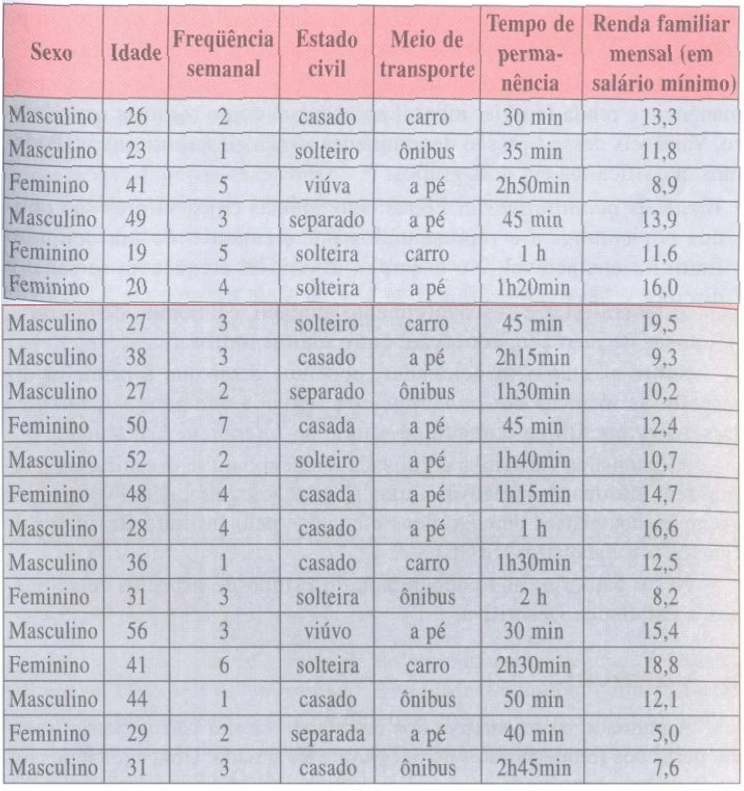
\includegraphics[scale=0.5]{figuras/fig104.png}	
	\end{center}
	
	\item construa a tabela de frequência da variável sexo.
	
	\item Construa uma tabela de frequência para a variável frequência semanal de visitas ao parque.

	\item Com os dados referentes à idade agrupados em classes de intervalo, cada um com amplitude igual a 10, construa uma tabela de frequência.
	
	\item Em uma pesquisa socioeconômica sobre itens de conforto, perguntou-se a cada um dos 800 entrevistados: Quantos aparelhos de TV em cores há em sua casa?
	
	Os resultados aparecem na tabela:
	
	\begin{center}
		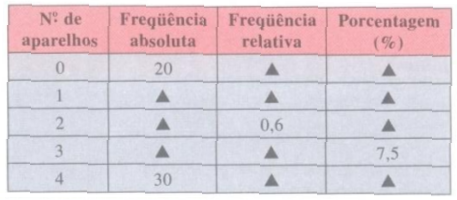
\includegraphics[scale=0.7]{figuras/fig105.png}
	\end{center}
	
	\begin{enumerate}[a)]
		\item Complete a tabela.
		\item Suponha que levantamentos posteriores mostraram que os resultados dessa amostra representam, em termos da frequência relativa, a distribuição do número de aparelhos de TV de toda a população. No universo de 680 000 domicílios, qual o número daqueles em que há exatamente 1 aparelho?
	\end{enumerate}
	
	\item Os dados seguintes referem-se ao tempo de espera (em minutos) de 30 clientes em uma fila de banco, em um dia de grande movimento:
	
	\begin{center}
	\begin{tabular}{cccccccccc}
	\hline 
	23 & 19 & 7 & 21 & 16 & 13 & 11 & 16 & 33 & 22 \\ 
	\hline 
	17 & 15 & 12 & 18 & 25 & 20 & 14 & 16 & 12 & 10 \\ 
	\hline 
	8 & 20 & 16 & 14 & 19 & 23 & 36 & 30 & 28 & 35 \\ 
	\hline 
	\end{tabular} 
	\end{center}
	
	Construa uma tabela de frequência, agrupando as informações em classes de amplitude igual a 5, a partir do menor tempo encontrado.
	
	\item A tabela abaixo informa os tipos de lazer preferidos por 80 garotos da 1ª série do ensino médio de um colégio.
	
	\begin{center}
	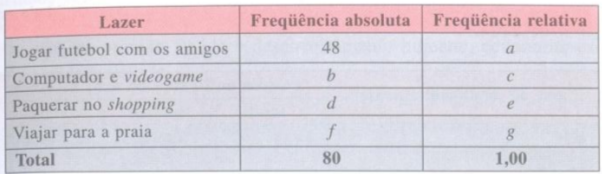
\includegraphics[scale=0.7]{figuras/fig106.png}
	\end{center}
	
	Complete a tabela, sabendo que \textit{c} é o dobro de \textit{e}, que é o quíntuplo de \textit{g}.
	
	\item Vinte e cinco jovens de até 15 anos foram selecionados para participar de um programa de desenvolvido pela Secretaria de Esportes de uma cidade cujo objetivo consiste na formação de futuros jogadores de vôlei. As alturas dos jovens (em metros) são dadas a segui:
	
	\begin{center}
	\begin{tabular}{ccccccccc}
	\hline 
	1,82 & 1,77 & 1,79 & 1,74 & 1,73 & 1,81 & 1,82 & 1,69 & 1,71 \\ 
	\hline 
	1,78 & 1,78 & 1,88 & 1,72 & 1,65 & 1,75 & 1,78 & 1,73 &   \\ 
	\hline 
	1,82 & 1,84 & 1,74 & 1,76 & 1,79 & 1,83 & 1,76 & 1,7 &   \\ 
	\hline 
	\end{tabular} 
	\end{center}
	
	\begin{enumerate}[a)]
		\item A partir de menor altura encontrada, agrupe os dados em classes de amplitude 5 cm e faça a tabela de frequência correspondente.
		\item Em visita ao centro de treinamento, um técnico estrangeiro sugeriu que pelo menos 48\% dos jovens deveriam ter estatura superior ou igual a 1,80 m. Quantos jovens nessas condições deve ser incorporados ao atual grupo, de acordo com tal sugestão? Use os dados agrupados no item \textit{a}.
	\end{enumerate}
	
	\item A tabela seguinte informa os valores de 160 empréstimos solicitados a um banco por pessoas físicas durante uma semana.
	
	\begin{center}
		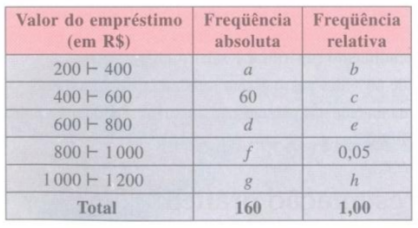
\includegraphics[scale=0.7]{figuras/fig107.png}
	\end{center}
	
	Complete a tabela, sabendo que 52,5\% dos empréstimos representavam valores maiores ou iguais a R\$ 600,00 e que entre eles, $\dfrac{2}{3}$ eram inferiores a R\$ 800,00.
	
	\item (UF-GO) A tabela abaixo foi extraída da Pesquisa Nacional por Amostra de Domicílio/2001 do IBGE. Ela mostra as classes de rendimento mensal no Estado de Goiás e o número de pessoas de 10 anos ou mais de idade em cada classe.
	
	\begin{center}
		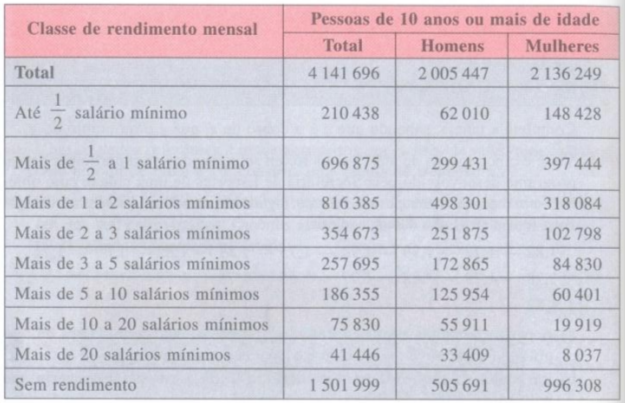
\includegraphics[scale=0.7]{figuras/fig108.png}
	\end{center}
	
	Analise essa tabela e julgue os itens a seguir:
	\begin{enumerate}[1)]
		\item O número de pessoas que ganham mais de 5 salários mínios é inferior a 8 \% do total de pessoas.
		\item A razão entre o número de mulheres e de homens que ganha até 1 salário mínimo é maior que a razão entre o número de mulheres e de homens com rendimento superior a 1 salário mínimo.
		\item Mais de 60\% das pessoas sem rendimento são mulheres.
		\item Mais da metade das pessoas não possuem rendimento ou ganham até 1 salário mínimo.
	\end{enumerate}	
\end{list}

\subsection{Representação Gráfica}
\begin{list}{\textbf{Questão \arabic{quest}.}}{\usecounter{quest}}
%define a margem da lista.	
%\setlength{\labelwidth}{-2mm} \setlength{\parsep}{0mm}
%\setlength{\topsep}{0mm} \setlength{\leftmargin}{-2mm}
\renewcommand{\labelenumi}{(\alph{enumi})}

	\item (Vunesp-SP) O gráfico, publicado pela revista \textit{Veja} de 28/07/1999, mostra como são divididos os 188 bilhões de reais do orçamento da União entre os setores de saúde, educação , previdência e outros.
	
	\begin{center}
		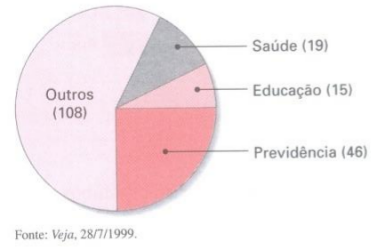
\includegraphics[scale=0.7]{figuras/fig109.png}
	\end{center}	
	
	Se os 46 bilhões de reais gastos com a previdência fosse totalmente repassados aos demais setores, de modo que 50\% fossem destinados à saúde, 40\% à edução e os 10\% restantes aos outros, determine o aumento que o setor de saúde teria:
	\begin{enumerate}[a)]
		\item em reais;
		\item em porcentagem, em relação à sua dotação inicial, aproximadamente.
	\end{enumerate}
	
	\item Uma pesquisa realizada com 800 pessoas às vésperas de um feriado prolongado tinha como pergunta principal: " O que você pretende fazer nesses quatro dias?". Os resultados são dados na tabela seguinte:
	
	\begin{center}
		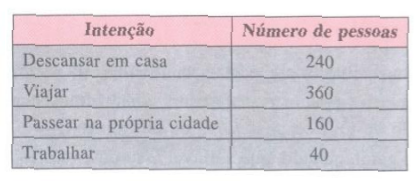
\includegraphics[scale=0.7]{figuras/fig110.png}
	\end{center}	
	
	Faça um gráfico de setores para representar esses resultados.
	
	\item Os gráfico seguintes mostram a disposição dos alunos das turmas da 3º série do ensino médio para fazer cursinho pré-vestibular paralelamente a frequentar as aluas do colégio.
	
	\begin{center}
		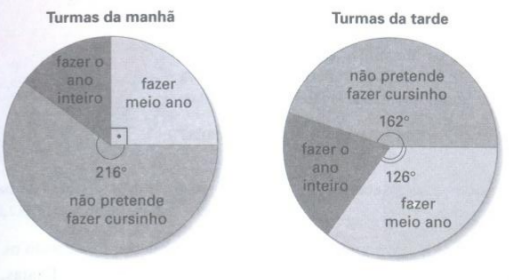
\includegraphics[scale=0.7]{figuras/fig111.png}
	\end{center}	
	
	Sabendo que as turmas da manhã contam com 340 alunos e as da tarde co 280 alunos, determine:
	\begin{enumerate}[a)]
		\item o número total de alunos que não pretendem fazer cursinho;
		\item a diferença entre o número de alunos do vespertino e do matutino que pretendam fazer cursinho o ano inteiro.
	\end{enumerate}
	
	\item Em uma cidade, o mercado de leite é disputado por quatro marcas: X, Y, Z e W. Os resultados de uma sondagem a propósito da marca preferida, realizada com 400 consumidores, estão parcialmente apresentados na tabela e no gráfico seguintes.
	
	\begin{center}
		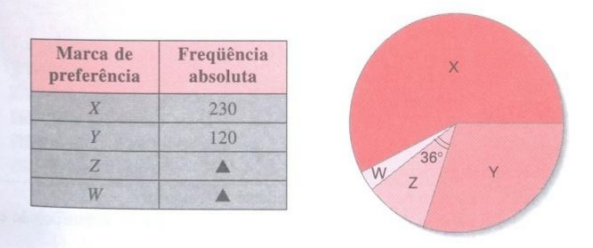
\includegraphics[scale=0.7]{figuras/fig112.png}
	\end{center}	
	
	Determine:
	\begin{enumerate}[a)]
		\item a diferença entre o número de consumidores que preferem Z a W;
		\item a diferença entre os ângulos correspondentes a X e Y.
	\end{enumerate}
	
	\item Uma psicóloga realizou com aos alunos da 1ª série do ensino médio de um colégio um estudo sobre orientação profissional. Após algumas dinâmicas e entrevistas, condensou as informações sobre a intenção de carreira dos alunos no gráfico abaixo. Quando os mesmos alunos estavam na 3ª série, a psicologa repetiu o estudo com eles e notou que, em relação à sondagem anterior, $\dfrac{5}{16}$ do interessados em Humanas migraram para Exatas e $\dfrac{3}{40}$ para Biológicas. Admitindo que não haja outras migrações:
	
	\begin{center}
		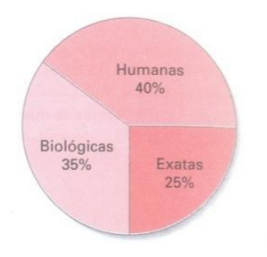
\includegraphics[scale=0.7]{figuras/fig113.png}
	\end{center}	
	
	\begin{enumerate}[a)]
		\item construa o novo gráfico de setores correspondente, destacando os ângulos;
		\item determine quantos alunos migraram de Humanas para Exatas, sabendo que o número dos participantes da dinâmica foi 400.
	\end{enumerate}
	
	\item Uma universidade realizou um levantamento sobre a origem dos 4.800 novos alunos ingressantes. Os dados encontram-se resumidos nos gráficos seguintes:
	
	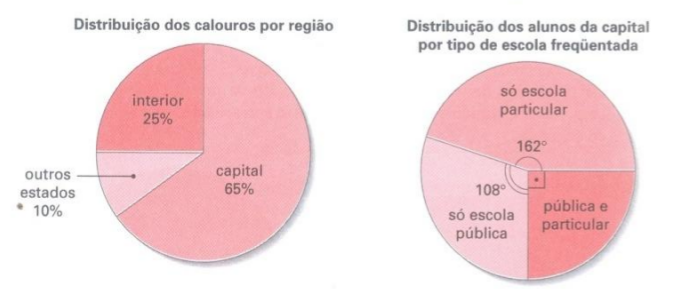
\includegraphics[scale=0.7]{figuras/fig114.png}
	
	Com base nos gráficos, responda:
	\begin{enumerate}[a)]
		\item Qual é o número de calouros procedentes do interior?
		\item Qual é o número de alunos da capital que estudaram no dois tipos de escola (pública e particular).?
		\item Qual é a porcentagem de calouros que estudaram em escolas particulares da capital?
		\item Qual é o número de calouros que já frequentaram a escola pública na capital?
	\end{enumerate}
\end{list}

%=============================================================================================================================
\subsection{Atividades extras}
\begin{list}{\textbf{Questão \arabic{quest}.}}{\usecounter{quest}}
%define a margem da lista.	
%\setlength{\labelwidth}{-2mm} \setlength{\parsep}{0mm}
%\setlength{\topsep}{0mm} \setlength{\leftmargin}{-2mm}
\renewcommand{\labelenumi}{(\alph{enumi})}

	\item Para facilitar um projeto de ampliação da rede de esgoto de uma certa região de uma cidade, as autoridades tomaram uma amostra de tamanho 50 dos 270 quarteirões que compõem a região e foram encontrados os seguintes números de \textit{\textbf{casas por quarteirão}}:
	\begin{center}
	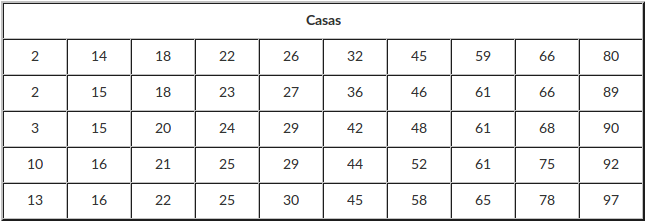
\includegraphics[scale=0.7]{figuras/fig115.png}
	\end{center}
	
	Determine a tabela de frequência.
	
	\item Organize os dados em forma de uma tabela de frequência:
	\begin{enumerate}[a)]
		\item As  cores  dos  20  primeiros  carros  que  passaram  em  uma  determinada  rua  foram 
anotadas, resultado os seguintes dados:
			\begin{center}
				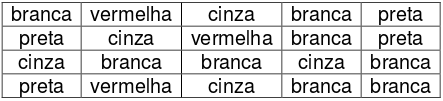
\includegraphics[scale=0.7]{figuras/fig116.png}
			\end{center}
		\item Uma  pesquisa  realizada  na  rua,  sobre  a  primeira  língua  estrangeira  que  a  pessoa 
tenha estudado, obteve os seguintes dados, coletados entre 50 pessoas entrevistadas:
			\begin{center}
				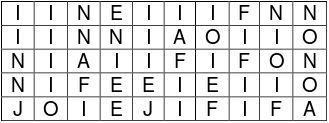
\includegraphics[scale=0.7]{figuras/fig117.png}
			\end{center}
		Onde I = Inglês, A = Alemão, E = Espanhol, J = Japonês, F = Francês N = Nenhuma e O = outra.
		
		\item Um dentista anotou o número de clientes atendidos por dia, durante um período de 30 dias, e obteve os seguintes dados:
			\begin{center}
				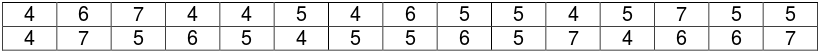
\includegraphics[scale=0.7]{figuras/fig118.png}
			\end{center}
		
		\item Numa  caixinha  de  fósforo,  vem  grafada  a  seguinte  informação:"contém  40  palitos". Para  verificar  esta  informação,  foram  adquiridas  60  caixinhas  de  fósforos  e  foi  feita uma  contagem  do  número  de  palitos  contidos  em  cada  uma  delas.  Os  resultados obtidos foram:
	\begin{center}
		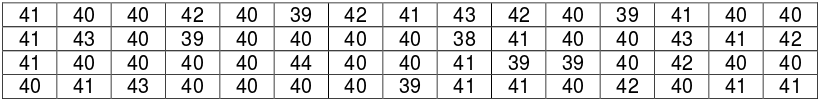
\includegraphics[scale=0.7]{figuras/fig119.png}
	\end{center}
	\end{enumerate}
	
	\item O conceito do 1º bimestre do ano de 2010, em Espanhol, de 35 alunos do 1º. ano do ensino médio B estão na seguinte tabela:
	\begin{center}
		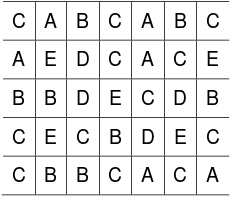
\includegraphics[scale=0.7]{figuras/fig120.png}
	\end{center}
	\begin{enumerate}[a)]
		\item Monte uma tabela de distribuição de frequência.
		\item Quando alunos obtiveram o conceito A ou B?
		\item[] Segundo os critérios abaixo responda o item c) e d)
			\begin{enumerate}
				\item[•] Conceito A,B ou C $-$ Aluno aprovado.
				\item[•] Conceito D $-$ Aluno em recuperação.
				\item[•] Conceito E $-$ Aluno reprovado.
			\end{enumerate}
		\item Qual a porcentagem de alunos que estão em recuperação?	
		\item Qual a porcentagem de alunos que NÃO estão em recuperação?	
	\end{enumerate}
	
	\item Um  questionário aplicado  a 1833  pessoas acima  de  20 anos sobre  a adição de uma determina  substância nos alimentos para a melhoria  do paladar,  principalmente para que esses alimentos fossem bem  aceitos entre  as  crianças, obteve  os seguintes resultados: 
	\begin{center}
		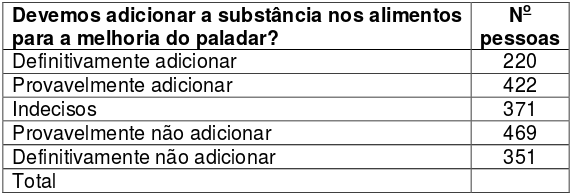
\includegraphics[scale=0.7]{figuras/fig121.png}
	\end{center}
	Complete a tabela de frequência acima e responda.
	\begin{enumerate}[a)]
		\item Qual o percentual de pessoas indecisas sobre a adição da  substância?
		\item Qual o percentual de pessoas que responderam entre \textit{definitivamente adicionar e provavelmente adicionar a substância}?
		\item Qual o percentual de pessoas que responderam entre \textit{provavelmente não adicionar e definitivamente não adicionar a substância}?
		\item Classifique a variável do estudo.
	\end{enumerate}
	
\end{list}